\phantomsection
\chapter*{প্রথম অধ্যায়ের নাম}
\addcontentsline{toc}{chapter}{প্রথম অধ্যায় (সূচীপত্রে)}
\markright{হেডার প্রথম}

\section*{(১)}
\addcontentsline{toc}{section}{(১) (সূচীপত্রে)}

জীবের মধ্যে সবচেয়ে সম্পূর্ণতা মানুষের। কিন্তু সবচেয়ে অসম্পূর্ণ হয়ে সে জন্মগ্রহণ করে। বাঘ ভালুক তার জীবনযাত্রার পনেরো- আনা মূলধন নিয়ে আসে প্রকৃতির মালখানা থেকে। জীবরঙ্গভূমিতে মানুষ এসে দেখা দেয় দুই শূন্য হাতে মুঠো বেঁধে।
মানুষ আসবার পূর্বেই জীবসৃষ্টিযজ্ঞে প্রকৃতির ভূরিব্যয়ের পালা শেষ হয়ে এসেছে। বিপুল মাংস, কঠিন বর্ম, প্রকাণ্ড লেজ নিয়ে জলে স্থলে পৃথুল দেহের যে অমিতাচার প্রবল হয়ে উঠেছিল তাতে ধরিত্রীকে দিলে ক্লান্ত করে। প্রমাণ হল আতিশয্যের পরাভব অনিবার্য। পরীক্ষায় এটাও স্থির হয়ে গেল যে, প্রশ্রয়ের পরিমাণ যত বেশি হয় দুর্বলতার বোঝাও তত দুর্বহ হয়ে ওঠে। নূতন পর্বে প্রকৃতি যথাসম্ভব মানুষের বরাদ্দ কম করে দিয়ে নিজে রইল নেপথ্যে।

মানুষকে দেখতে হল খুব ছোটো, কিন্তু সেটা একটা কৌশল মাত্র। এবারকার জীবযাত্রার পালায় বিপুলতাকে করা হল বহুলতায় পরিণত। মহাকায় জন্তু ছিল প্রকাণ্ড একলা, মানুষ হল দূরপ্রসারিত অনেক।

জীবের মধ্যে সবচেয়ে সম্পূর্ণতা মানুষের। কিন্তু সবচেয়ে অসম্পূর্ণ হয়ে সে জন্মগ্রহণ করে। বাঘ ভালুক তার জীবনযাত্রার পনেরো- আনা মূলধন নিয়ে আসে প্রকৃতির মালখানা থেকে। জীবরঙ্গভূমিতে মানুষ এসে দেখা দেয় দুই শূন্য হাতে মুঠো বেঁধে।

মানুষ আসবার পূর্বেই জীবসৃষ্টিযজ্ঞে প্রকৃতির ভূরিব্যয়ের পালা শেষ হয়ে এসেছে। বিপুল মাংস, কঠিন বর্ম, প্রকাণ্ড লেজ নিয়ে জলে স্থলে পৃথুল দেহের যে অমিতাচার প্রবল হয়ে উঠেছিল তাতে ধরিত্রীকে দিলে ক্লান্ত করে। প্রমাণ হল আতিশয্যের পরাভব অনিবার্য। পরীক্ষায় এটাও স্থির হয়ে গেল যে, প্রশ্রয়ের পরিমাণ যত বেশি হয় দুর্বলতার বোঝাও তত দুর্বহ হয়ে ওঠে। নূতন পর্বে প্রকৃতি যথাসম্ভব মানুষের বরাদ্দ কম করে দিয়ে নিজে রইল নেপথ্যে।

মানুষকে দেখতে হল খুব ছোটো, কিন্তু সেটা একটা কৌশল মাত্র। এবারকার জীবযাত্রার পালায় বিপুলতাকে করা হল বহুলতায় পরিণত। মহাকায় জন্তু ছিল প্রকাণ্ড একলা, মানুষ হল দূরপ্রসারিত অনেক।

\section*{(২)}
\addcontentsline{toc}{section}{(২) (সূচীপত্রে)}

জীবের মধ্যে সবচেয়ে সম্পূর্ণতা মানুষের। কিন্তু সবচেয়ে অসম্পূর্ণ হয়ে সে জন্মগ্রহণ করে। বাঘ ভালুক তার জীবনযাত্রার পনেরো- আনা মূলধন নিয়ে আসে প্রকৃতির মালখানা থেকে। জীবরঙ্গভূমিতে মানুষ এসে দেখা দেয় দুই শূন্য হাতে মুঠো বেঁধে।

মানুষ আসবার পূর্বেই জীবসৃষ্টিযজ্ঞে প্রকৃতির ভূরিব্যয়ের পালা শেষ হয়ে এসেছে। বিপুল মাংস, কঠিন বর্ম, প্রকাণ্ড লেজ নিয়ে জলে স্থলে পৃথুল দেহের যে অমিতাচার প্রবল হয়ে উঠেছিল তাতে ধরিত্রীকে দিলে ক্লান্ত করে। প্রমাণ হল আতিশয্যের পরাভব অনিবার্য। পরীক্ষায় এটাও স্থির হয়ে গেল যে, প্রশ্রয়ের পরিমাণ যত বেশি হয় দুর্বলতার বোঝাও তত দুর্বহ হয়ে ওঠে। নূতন পর্বে প্রকৃতি যথাসম্ভব মানুষের বরাদ্দ কম করে দিয়ে নিজে রইল নেপথ্যে।

মানুষকে দেখতে হল খুব ছোটো, কিন্তু সেটা একটা কৌশল মাত্র। এবারকার জীবযাত্রার পালায় বিপুলতাকে করা হল বহুলতায় পরিণত। মহাকায় জন্তু ছিল প্রকাণ্ড একলা, মানুষ হল দূরপ্রসারিত অনেক।
\begin{figure}
	\centering
	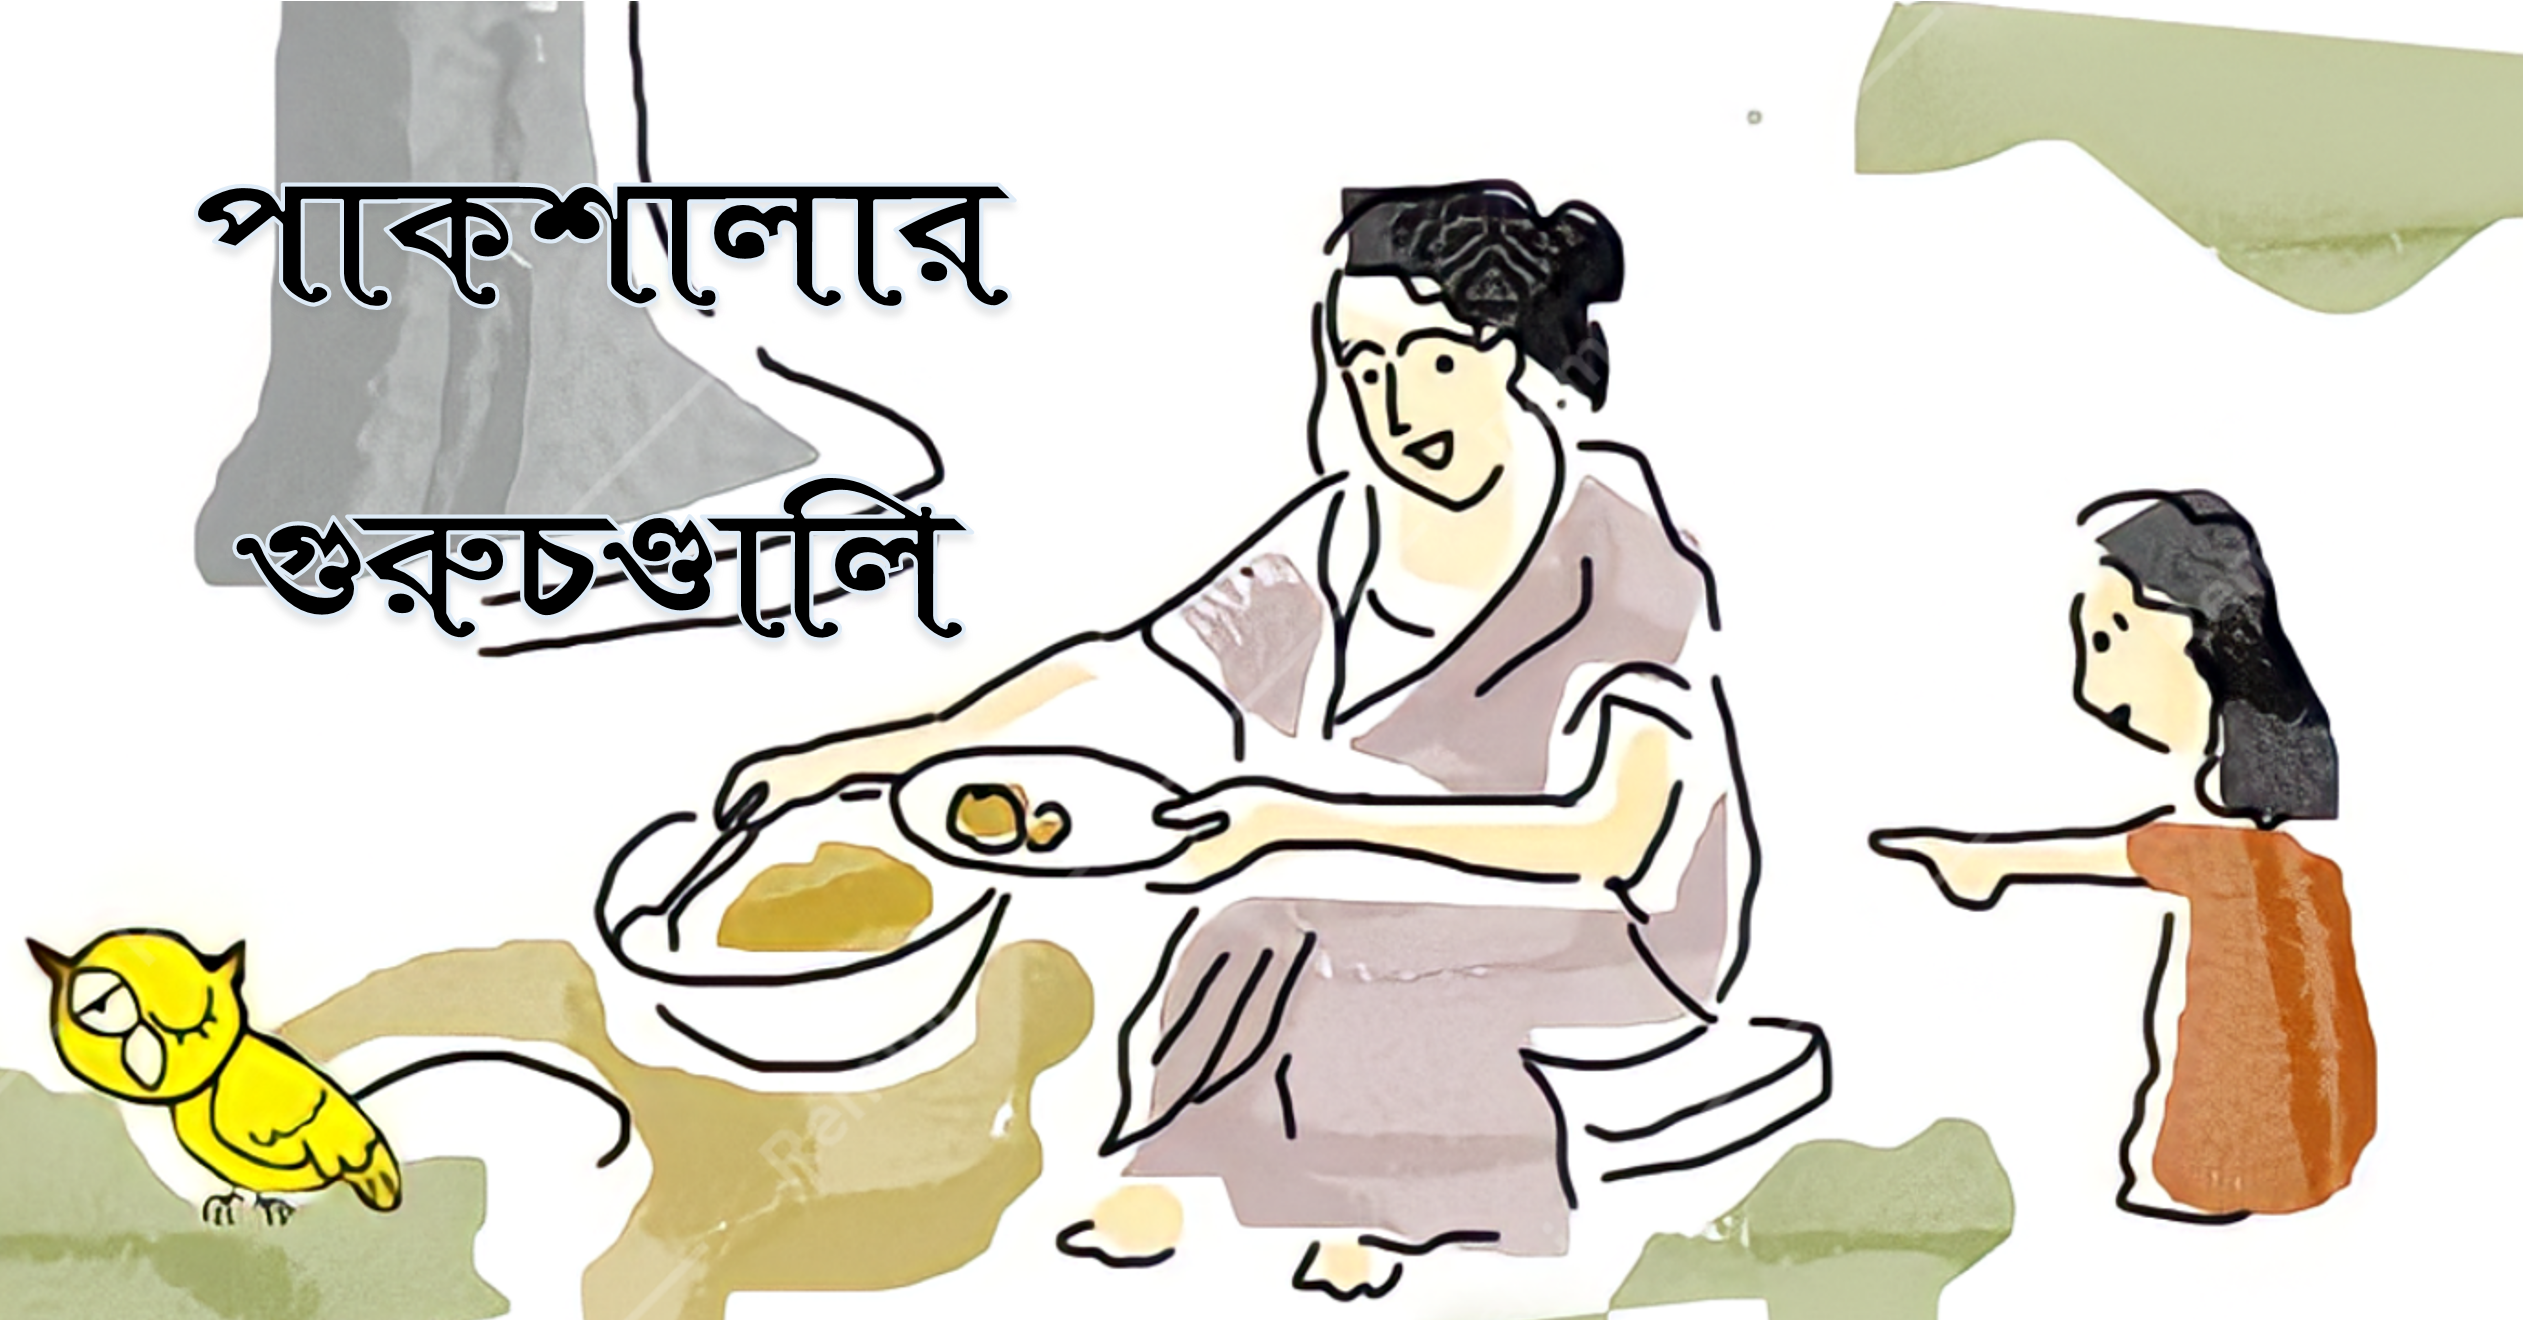
\includegraphics[width=\linewidth]{Images/DemoPic1.png}
	\caption{\small \textbf{ডেমো ক্যাপশন}}
\end{figure}

জীবের মধ্যে সবচেয়ে সম্পূর্ণতা মানুষের। কিন্তু সবচেয়ে অসম্পূর্ণ হয়ে সে জন্মগ্রহণ করে। বাঘ ভালুক তার জীবনযাত্রার পনেরো- আনা মূলধন নিয়ে আসে প্রকৃতির মালখানা থেকে। জীবরঙ্গভূমিতে মানুষ এসে দেখা দেয় দুই শূন্য হাতে মুঠো বেঁধে।

মানুষ আসবার পূর্বেই জীবসৃষ্টিযজ্ঞে প্রকৃতির ভূরিব্যয়ের পালা শেষ হয়ে এসেছে। বিপুল মাংস, কঠিন বর্ম, প্রকাণ্ড লেজ নিয়ে জলে স্থলে পৃথুল দেহের যে অমিতাচার প্রবল হয়ে উঠেছিল তাতে ধরিত্রীকে দিলে ক্লান্ত করে। প্রমাণ হল আতিশয্যের পরাভব অনিবার্য। পরীক্ষায় এটাও স্থির হয়ে গেল যে, প্রশ্রয়ের পরিমাণ যত বেশি হয় দুর্বলতার বোঝাও তত দুর্বহ হয়ে ওঠে। নূতন পর্বে প্রকৃতি যথাসম্ভব মানুষের বরাদ্দ কম করে দিয়ে নিজে রইল নেপথ্যে।

মানুষকে দেখতে হল খুব ছোটো, কিন্তু সেটা একটা কৌশল মাত্র। এবারকার জীবযাত্রার পালায় বিপুলতাকে করা হল বহুলতায় পরিণত। মহাকায় জন্তু ছিল প্রকাণ্ড একলা, মানুষ হল দূরপ্রসারিত অনেক। 
\begin{quotation}
	\textit{জীবের মধ্যে সবচেয়ে সম্পূর্ণতা মানুষের। কিন্তু সবচেয়ে অসম্পূর্ণ হয়ে সে জন্মগ্রহণ করে। বাঘ ভালুক তার জীবনযাত্রার পনেরো- আনা মূলধন নিয়ে আসে প্রকৃতির মালখানা থেকে। জীবরঙ্গভূমিতে মানুষ এসে দেখা দেয় দুই শূন্য হাতে মুঠো বেঁধে।\\
	মানুষ আসবার পূর্বেই জীবসৃষ্টিযজ্ঞে প্রকৃতির ভূরিব্যয়ের পালা শেষ হয়ে এসেছে। বিপুল মাংস, কঠিন বর্ম, প্রকাণ্ড লেজ নিয়ে জলে স্থলে পৃথুল দেহের যে অমিতাচার প্রবল হয়ে উঠেছিল তাতে ধরিত্রীকে দিলে ক্লান্ত করে। প্রমাণ হল আতিশয্যের পরাভব অনিবার্য। পরীক্ষায় এটাও স্থির হয়ে গেল যে, প্রশ্রয়ের পরিমাণ যত বেশি হয় দুর্বলতার বোঝাও তত দুর্বহ হয়ে ওঠে। নূতন পর্বে প্রকৃতি যথাসম্ভব মানুষের বরাদ্দ কম করে দিয়ে নিজে রইল নেপথ্যে।\\
	মানুষকে দেখতে হল খুব ছোটো, কিন্তু সেটা একটা কৌশল মাত্র। এবারকার জীবযাত্রার পালায় বিপুলতাকে করা হল বহুলতায় পরিণত। মহাকায় জন্তু ছিল প্রকাণ্ড একলা, মানুষ হল দূরপ্রসারিত অনেক।}
\end{quotation}
জীবের মধ্যে সবচেয়ে সম্পূর্ণতা মানুষের। কিন্তু সবচেয়ে অসম্পূর্ণ হয়ে সে জন্মগ্রহণ করে। বাঘ ভালুক তার জীবনযাত্রার পনেরো- আনা মূলধন নিয়ে আসে প্রকৃতির মালখানা থেকে। জীবরঙ্গভূমিতে মানুষ এসে দেখা দেয় দুই শূন্য হাতে মুঠো বেঁধে।

মানুষ আসবার পূর্বেই জীবসৃষ্টিযজ্ঞে প্রকৃতির ভূরিব্যয়ের পালা শেষ হয়ে এসেছে। বিপুল মাংস, কঠিন বর্ম, প্রকাণ্ড লেজ নিয়ে জলে স্থলে পৃথুল দেহের যে অমিতাচার প্রবল হয়ে উঠেছিল তাতে ধরিত্রীকে দিলে ক্লান্ত করে। প্রমাণ হল আতিশয্যের পরাভব অনিবার্য। পরীক্ষায় এটাও স্থির হয়ে গেল যে, প্রশ্রয়ের পরিমাণ যত বেশি হয় দুর্বলতার বোঝাও তত দুর্বহ হয়ে ওঠে। নূতন পর্বে প্রকৃতি যথাসম্ভব মানুষের বরাদ্দ কম করে দিয়ে নিজে রইল নেপথ্যে।

মানুষকে দেখতে হল খুব ছোটো, কিন্তু সেটা একটা কৌশল মাত্র। এবারকার জীবযাত্রার পালায় বিপুলতাকে করা হল বহুলতায় পরিণত। মহাকায় জন্তু ছিল প্রকাণ্ড একলা, মানুষ হল দূরপ্রসারিত অনেক।

\vskip 30pt
\scriptsize
	\textbf{সূত্র:}
	\begin{enumerate}%[label={}]
		\item ১২০৫-১২০৬ খ্রিস্টাব্দের দিকে ইখতিয়ার উদ্দিন মুহম্মদ বখতিয়ার খলজী নামের একজন তুর্কী বংশোদ্ভূত সেনাপতি রাজা লক্ষ্মণ সেনকে পরাজিত করে সেন রাজবংশের পতন ঘটান।
		\item ১৭৫৭ খ্রিস্টাব্দে ব্রিটিশ ইস্ট ইন্ডিয়া কোম্পানি পলাশীর যুদ্ধে জয়লাভের মাধ্যমে বাংলার শাসনক্ষমতা দখল করে
		\item ১৮৫৭ খ্রিস্টাব্দের সিপাহী বিপ্লবের পর কোম্পানির হাত থেকে বাংলার শাসনভার ব্রিটিশ সাম্রাজ্যের সরাসরি নিয়ন্ত্রণে আসে
		\item ভারতীয় উপমহাদেশের দেশভাগের সময় ১৯৪৭ খ্রিস্টাব্দে ধর্ম গরিষ্ঠতার ভিত্তিতে পুনর্বার বাংলা প্রদেশটিকে ভাগ করা হয়। পাকিস্তান এর প্রদেশ হিসাবে জন্ম নেয় পূর্ব পাকিস্তান 
		\item ১৯৭১ সালে ৯ মাস ব্যাপী রক্তক্ষয়ী যুদ্ধের মাধ্যমে পাকিস্তানী হানাদার বাহিনীকে পরাজিত করে স্বাধীনতা লাভ করে বাংলাদেশ 
	\end{enumerate}


